\section{Ventas y cotizaciones (Nivel Experto)}

El módulo de Ventas es donde formalizas los presupuestos (cotizaciones) que le enviarás al cliente y los conviertes en ventas confirmadas (pedidos) cuando pagan. En esta sección aprenderás cada detalle de la pantalla de Ventas para que domines todas sus opciones.

% ─────────────────────────────────────────────────────────────────────────────
\subsection{1. La pantalla principal de Ventas}

\begin{figure}[H]
    \centering
    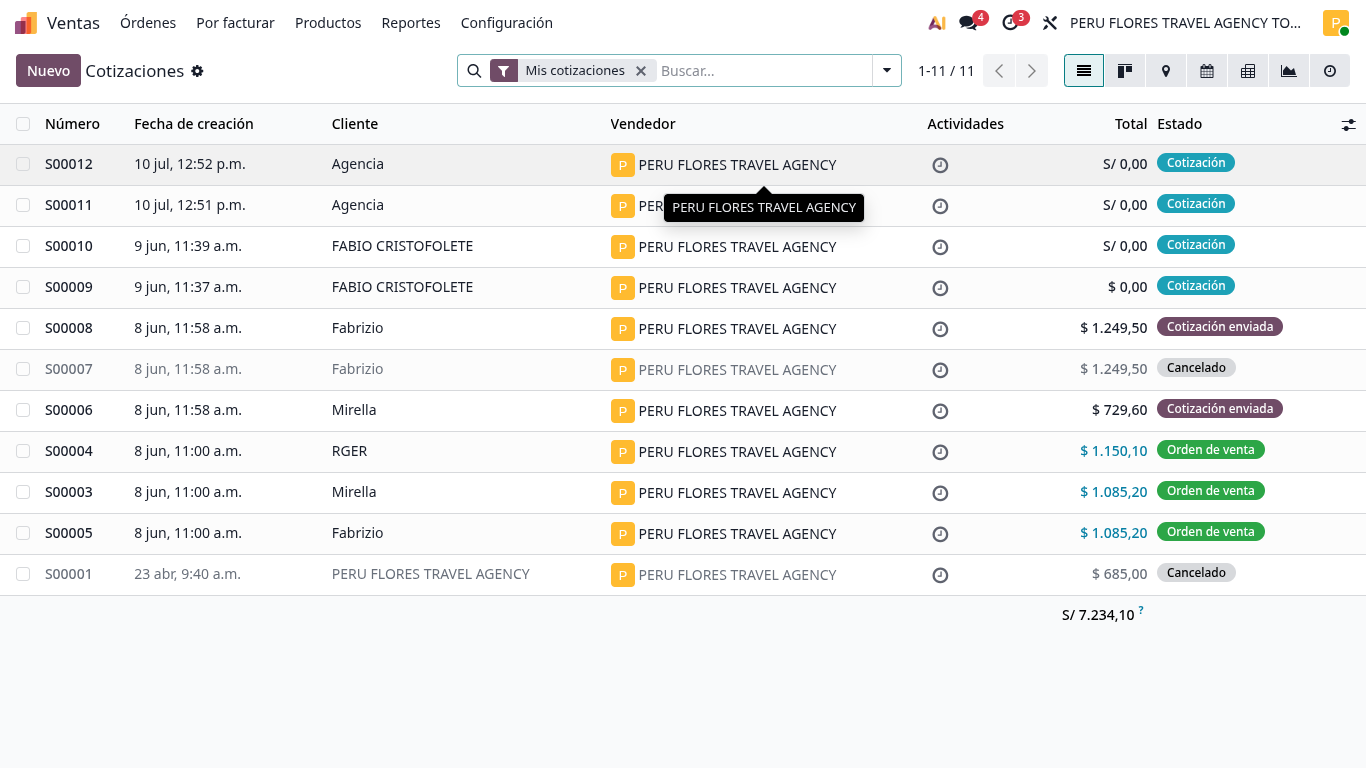
\includegraphics[width=0.9\textwidth]{assets/ven_g1_lista.png}
    \caption{Lista principal. Muestra el historial completo de cotizaciones y pedidos.}
\end{figure}

Al entrar al módulo de Ventas, verás tu lista de documentos. Odoo te permite buscar rápidamente cualquier cotización si recuerdas el nombre del cliente o el número de documento.

\begin{figure}[H]
    \centering
    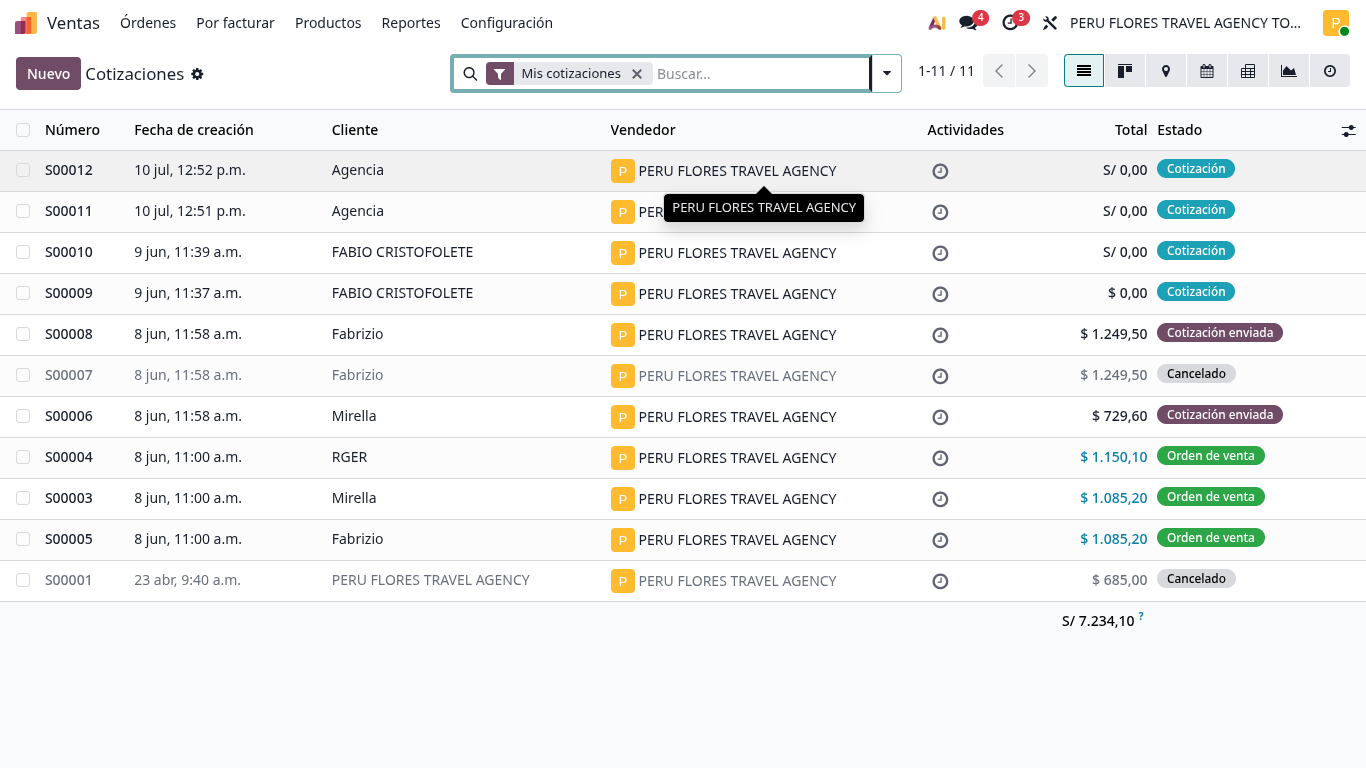
\includegraphics[width=0.9\textwidth]{assets/ven_g2_busqueda.png}
    \caption{La barra de búsqueda avanzada en la parte superior derecha.}
\end{figure}

Usa esta barra (marcada en rojo) para filtrar, por ejemplo, solo "Mis cotizaciones" o agruparlas por "Cliente".

% ─────────────────────────────────────────────────────────────────────────────
\subsection{2. Iniciar una nueva cotización}

Para crear un nuevo documento, haz clic en el botón \textbf{``Nuevo''}. Esto abrirá un formulario en blanco con muchísimas opciones que vamos a desglosar una a una.

\begin{figure}[H]
    \centering
    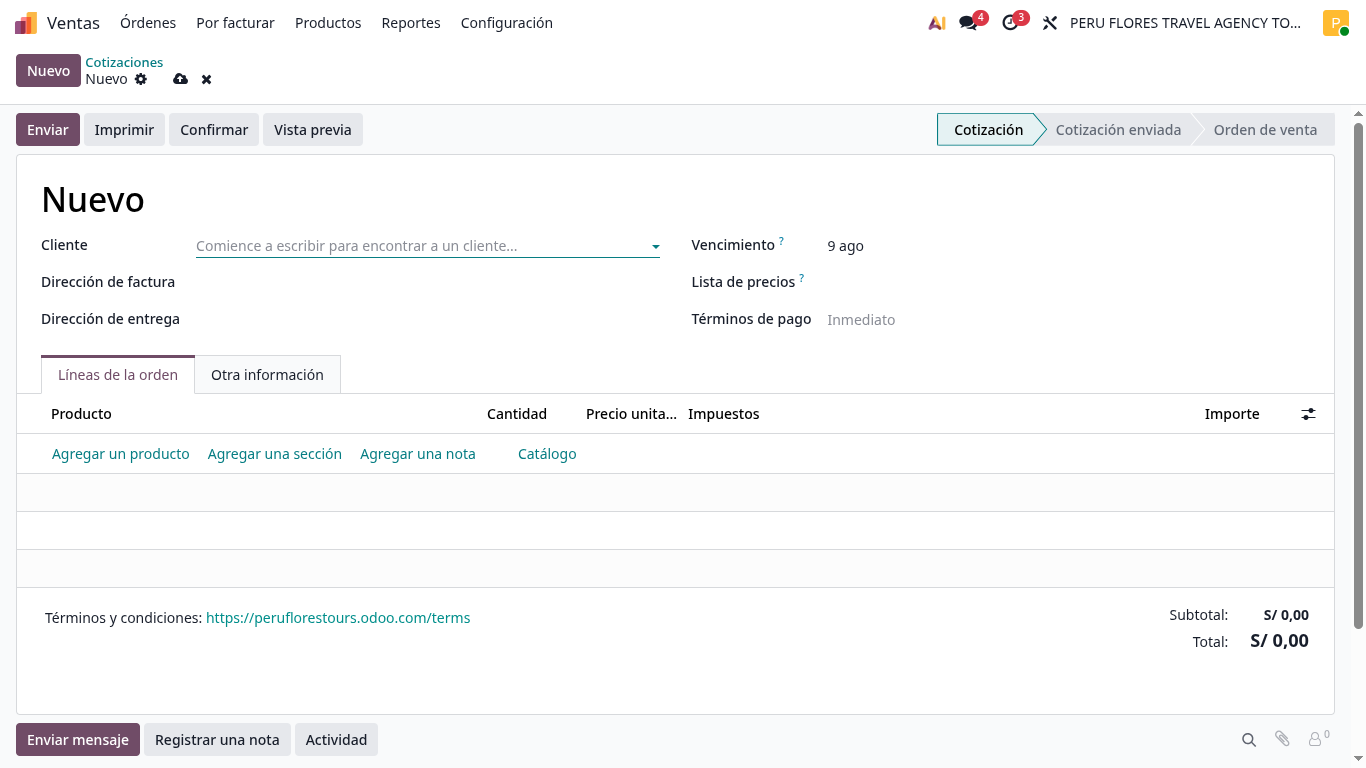
\includegraphics[width=0.9\textwidth]{assets/ven_g3_form.png}
    \caption{El formulario de cotización en blanco. A simple vista parece complejo, pero es muy ordenado.}
\end{figure}

\begin{figure}[H]
    \centering
    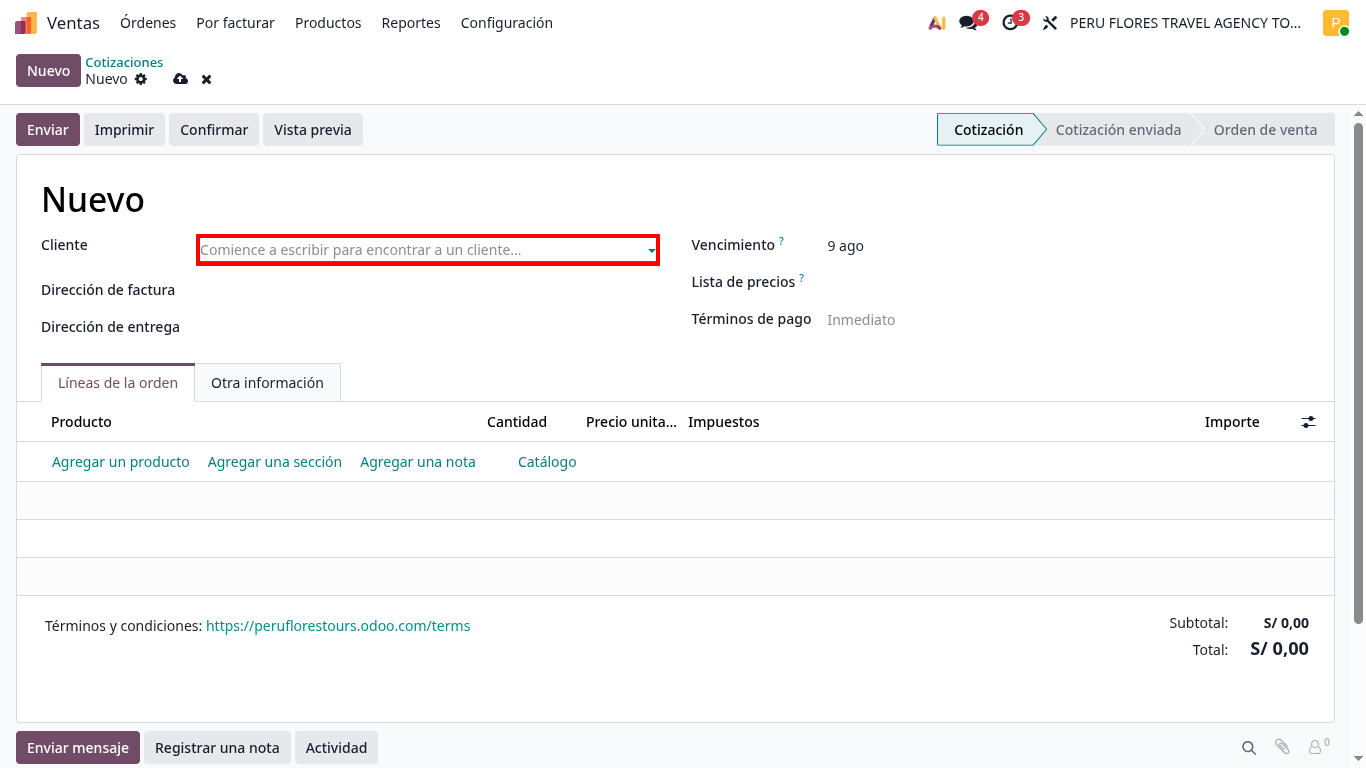
\includegraphics[width=0.9\textwidth]{assets/ven_g6_cliente.png}
    \caption{Campo del cliente (marcado en rojo). Es lo primero que debes llenar.}
\end{figure}

\textbf{Paso A: Elegir al cliente}
En el campo marcado arriba, escribe el nombre del pasajero. Automáticamente jalará su información de contacto (correo, teléfono).

\begin{figure}[H]
    \centering
    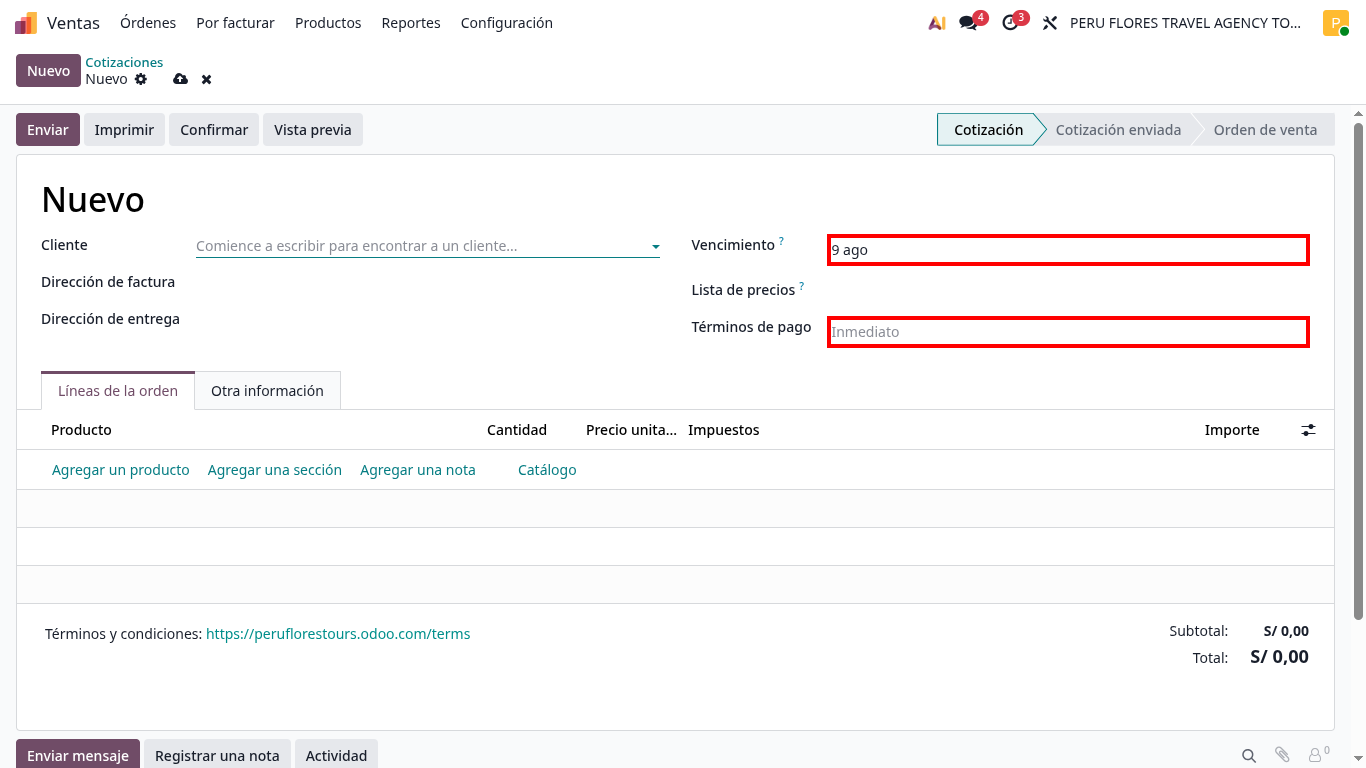
\includegraphics[width=0.9\textwidth]{assets/ven_g7_fechas_pago.png}
    \caption{Configuración de Expiración y Plazos de pago.}
\end{figure}

\textbf{Paso B: Fechas importantes}
Justo debajo del cliente, puedes establecer cuándo vence la cotización (ej. válida por 5 días) y los plazos de pago (ej. 50\% adelanto, 50\% a la llegada).

% ─────────────────────────────────────────────────────────────────────────────
\subsection{3. Agregar los Tours (Líneas de pedido)}

\begin{figure}[H]
    \centering
    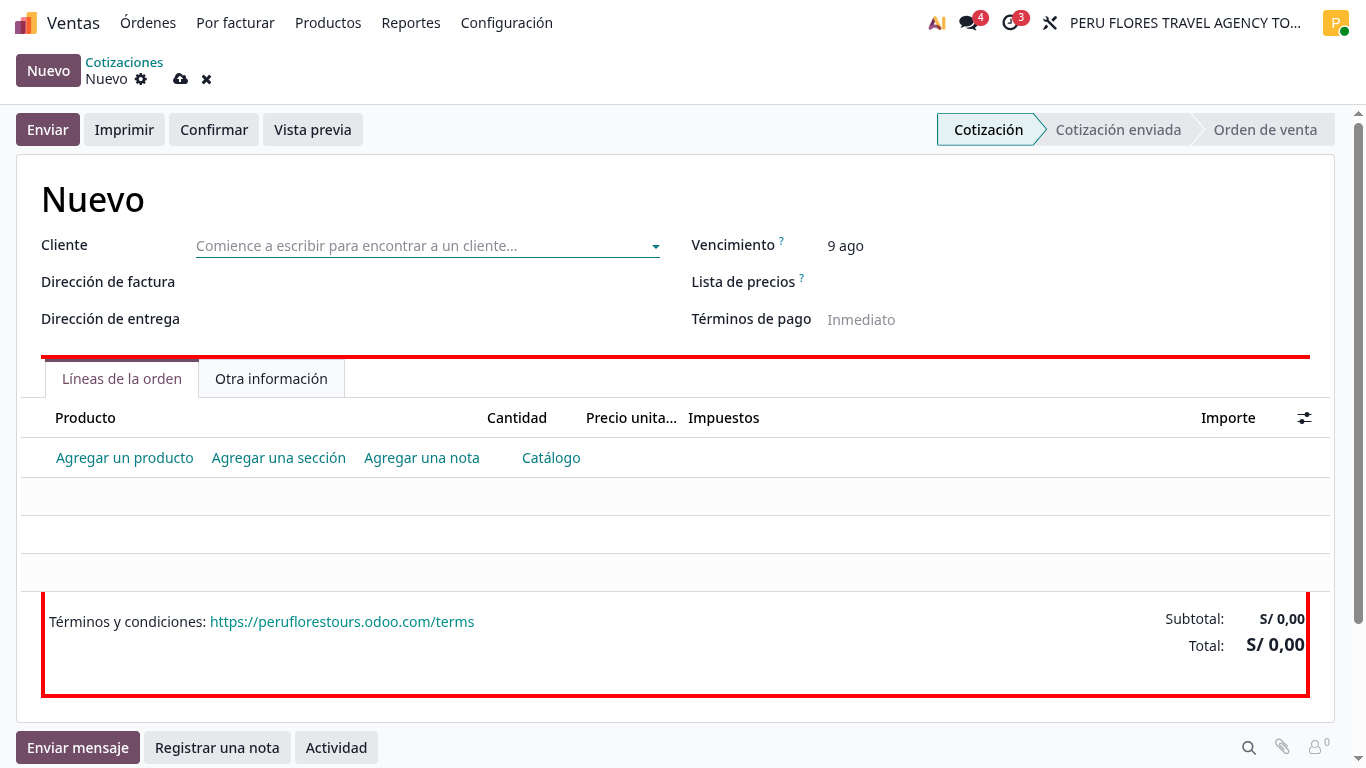
\includegraphics[width=0.9\textwidth]{assets/ven_g8_pestanas.png}
    \caption{La zona de pestañas, dominada por ``Líneas de pedido''.}
\end{figure}

En la pestaña central (marcada en rojo) haz clic en \textbf{``Agregar un producto''} y busca el tour que el cliente desea. Asegúrate de revisar la columna de \textbf{Cantidad} y \textbf{Precio Unitario}. El sistema calculará el IGV o los impuestos configurados en la parte inferior.

% ─────────────────────────────────────────────────────────────────────────────
\subsection{4. Los botones de Acción (Enviar y Confirmar)}

Una vez que la cotización está llena, la atención pasa a la esquina superior izquierda.

\begin{figure}[H]
    \centering
    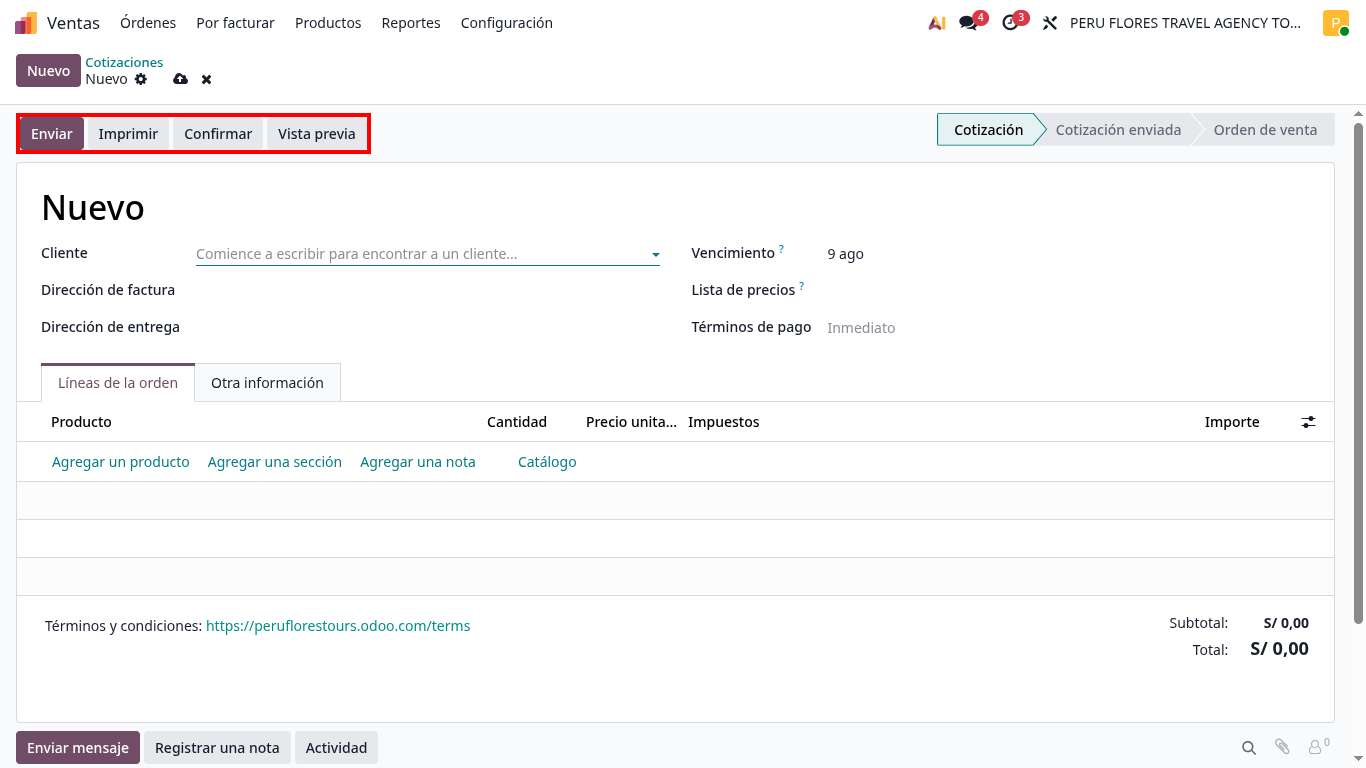
\includegraphics[width=0.9\textwidth]{assets/ven_g4_botones_accion.png}
    \caption{Los botones principales de acción.}
\end{figure}

\begin{figure}[H]
    \centering
    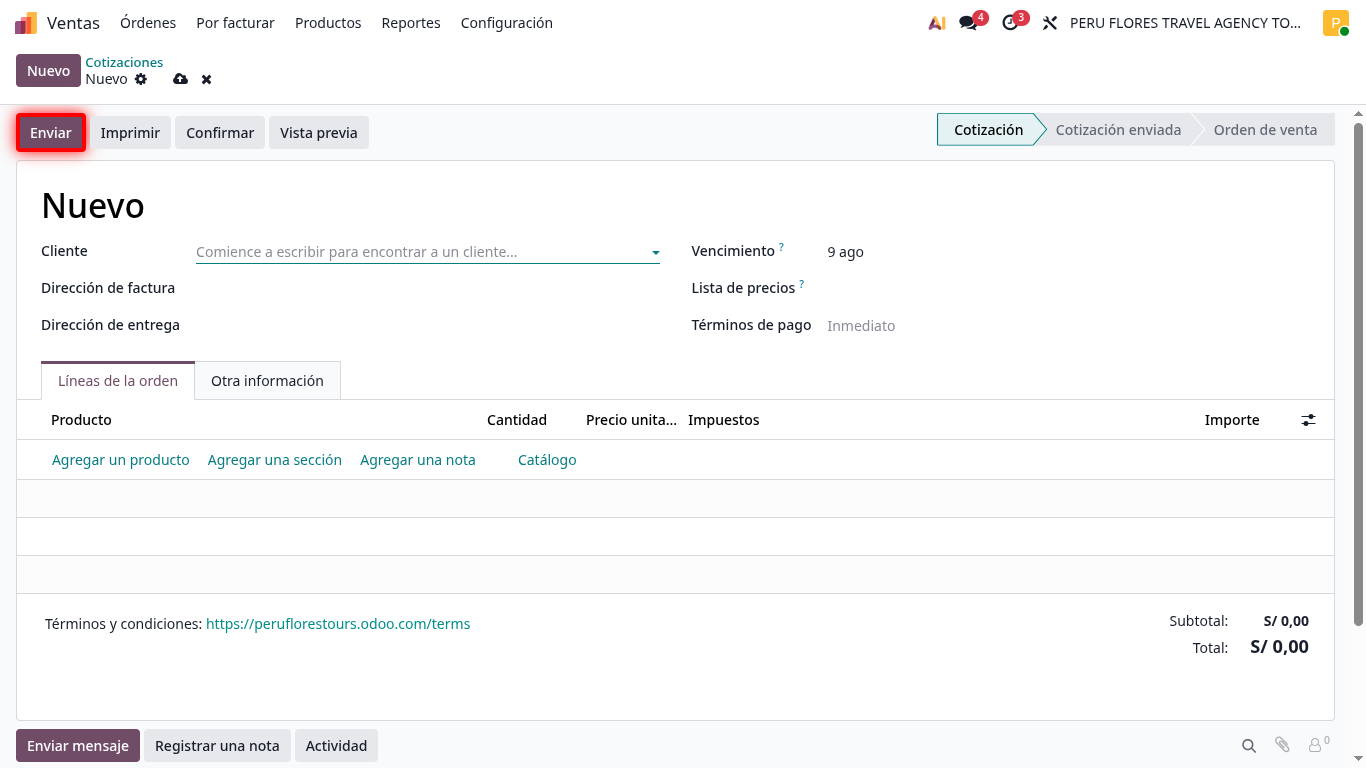
\includegraphics[width=0.9\textwidth]{assets/ven_06_enviar_correo_highlight_real.png}
    \caption{Botón para enviar la proforma por email directamente desde Odoo.}
\end{figure}

Haz clic en \textbf{``Enviar por correo electrónico''} para mandar el presupuesto oficial en PDF. El sistema te abrirá una ventana para que edites el mensaje si lo deseas.

\begin{figure}[H]
    \centering
    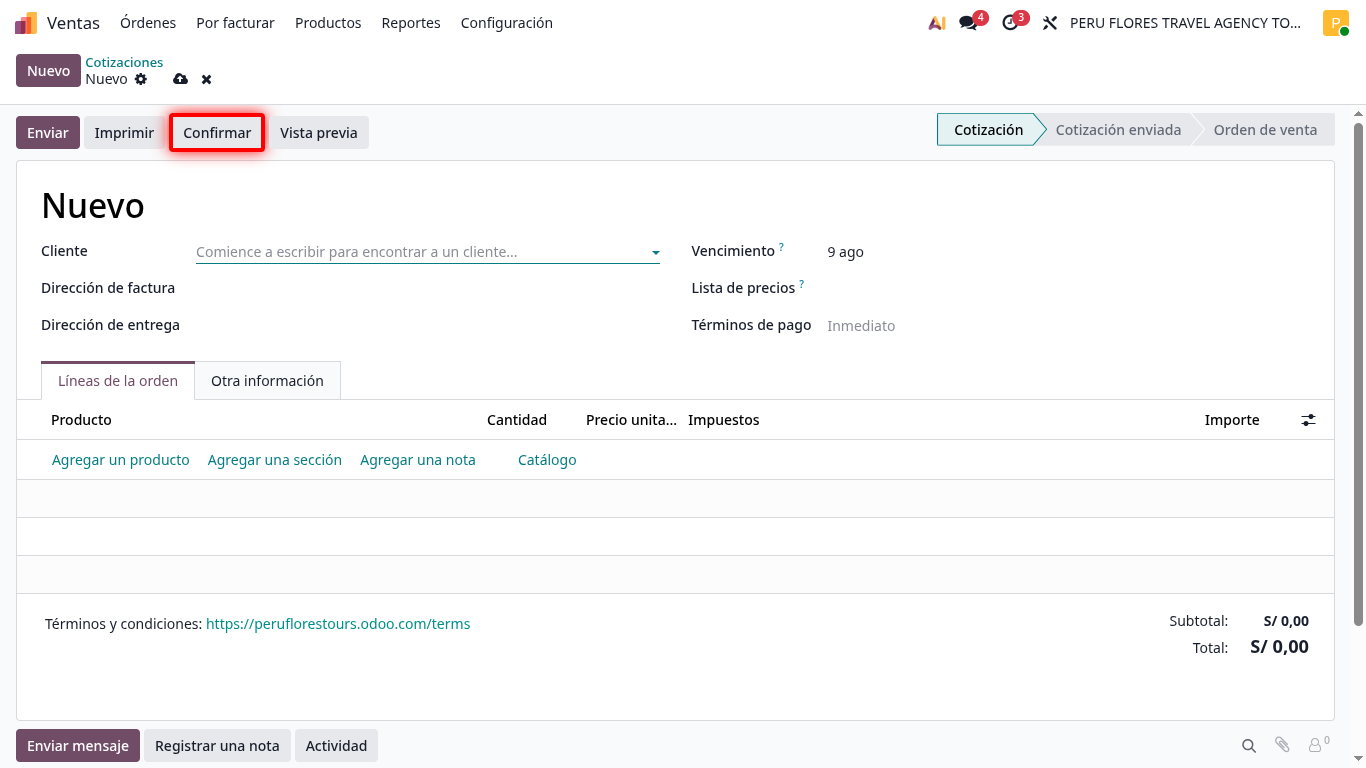
\includegraphics[width=0.9\textwidth]{assets/ven_07_confirmar_highlight_real.png}
    \caption{El botón de confirmación de venta.}
\end{figure}

Cuando el cliente te pague o confirme el viaje, vuelve a esta pantalla y haz clic en \textbf{``Confirmar''}. ¡Esto convierte tu cotización en una venta real (Pedido)!

% ─────────────────────────────────────────────────────────────────────────────
\subsection{5. La Barra de Estados}

¿Cómo sabes en qué etapa está tu venta sin leer todo el documento? Mirando la esquina superior derecha.

\begin{figure}[H]
    \centering
    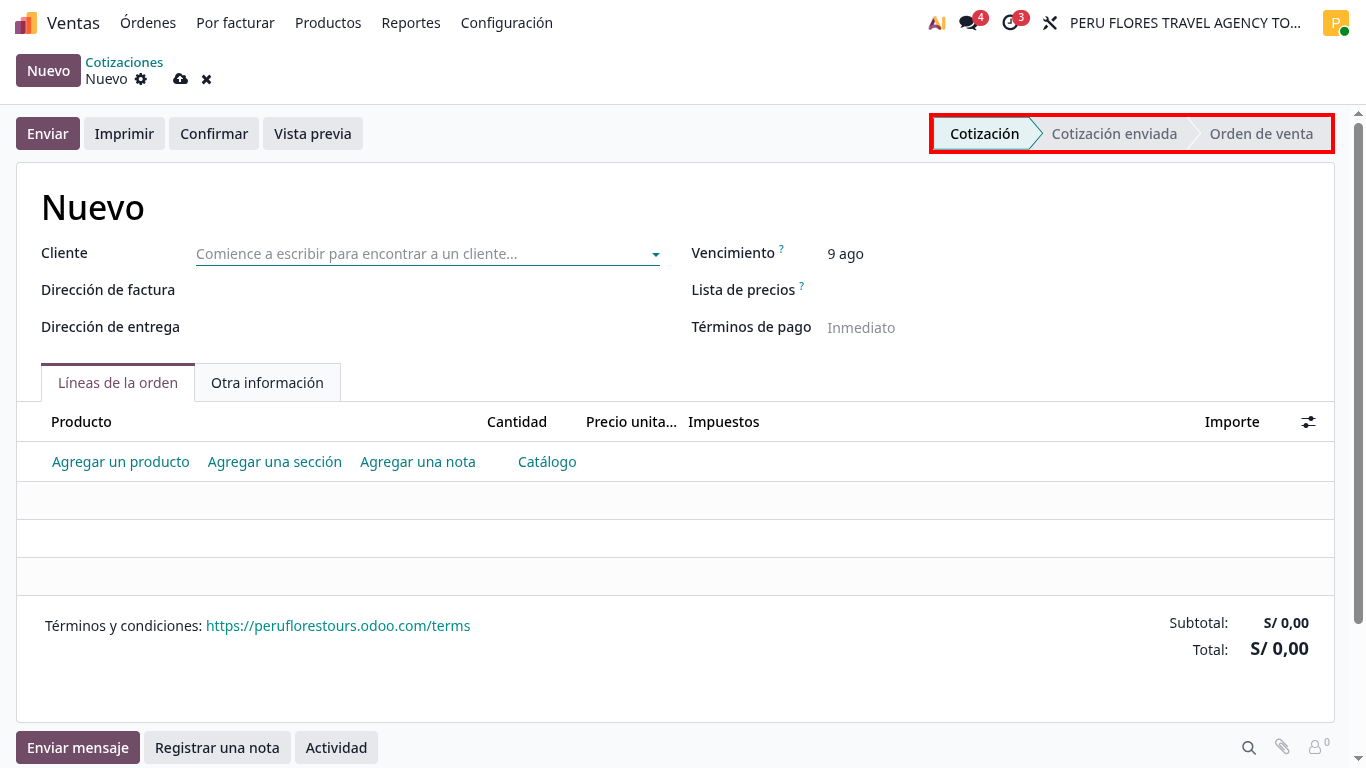
\includegraphics[width=0.9\textwidth]{assets/ven_g5_estado.png}
    \caption{La barra de estado del documento.}
\end{figure}

Esta barra avanzará desde \textbf{Presupuesto} (borrador), pasará a \textbf{Presupuesto enviado} (cuando mandas el correo) y terminará en \textbf{Pedido de Venta} (cuando confirmas).

% ─────────────────────────────────────────────────────────────────────────────
\subsection{6. El Historial de comunicaciones (Chatter)}

Odoo guarda todo lo que pasa con esta venta en un panel lateral o inferior llamado Chatter.

\begin{figure}[H]
    \centering
    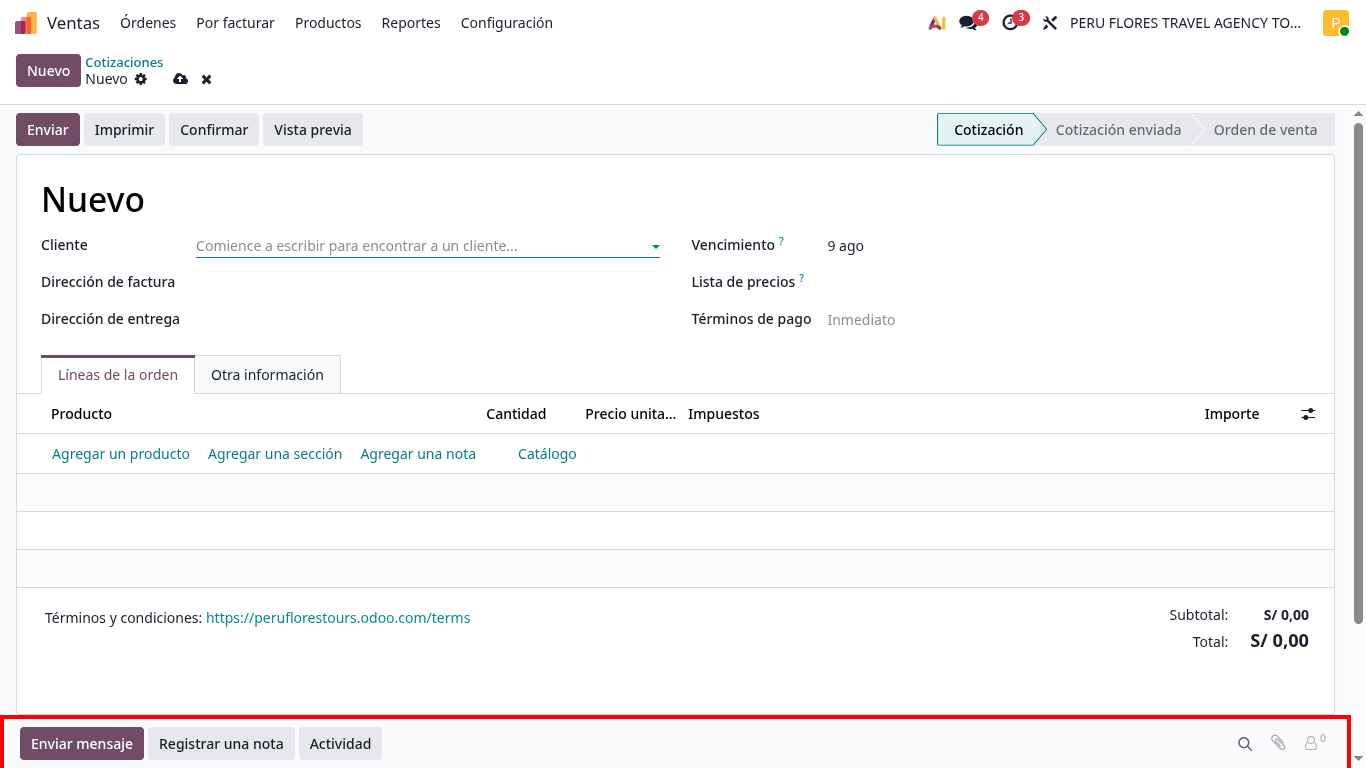
\includegraphics[width=0.9\textwidth]{assets/ven_g10_chatter.png}
    \caption{El Chatter guarda todo el historial de correos enviados, PDFs generados y notas internas.}
\end{figure}

Si en algún momento dudas si le enviaste la proforma al cliente, revisa este historial. Ahí quedará registrado el día, la hora y una copia del PDF que se le mandó. También puedes usar \textbf{``Registrar nota''} para dejar mensajes que el cliente no verá, solo tus compañeros de trabajo.
